\chapter{Arquitectura}
\label{chap:arquitectura}


En este capítulo se mostrarán los resultados obtenidos al aplicar la metodología descrita en la sección \ref{chap:metodo} a través de un enfoque top-down, comenzando con una descripción general, continuando con las decisiones
de diseño y terminando con los detalles de implementación. 

\section{Descripción general}
\section{Módulo de captura}
El módulo de captura de vídeo se encarga de crear y proporcionar fuentes de vídeo de diversa naturaleza para dar soporte al submódulo de registro (ver Sección 5.5), y al submódulo de representación 2D (ver Sección 5.3.4).
Es capaz de dar soporte multicámara. Se pueden crear tantas fuentes de vídeo como se disponga en el sistema, que será de alguno de los siguientes tipos: 
\begin{itemize}
\item RaspiCam: Para un rendimiento óptimo en la raspberry pi, al menos la cámara principal debería ser de este tipo.
\item Cámara USB: En caso de no disponer de una raspicam o si se quieren incluir cámara adicionales para obtener capturas desde otra posición (videoconferencia,...).
\end{itemize}

El submódulo de vídeo se implementa en dos componentes: el VideoFactory, que proporciona la interfaz de creación y gestión de fuentes de vídeo, y el VideoSource, que implementa una única fuente de vídeo basada en la biblioteca de visión artificial OpenCV.

OpenCV utiliza la clase cv::VideoCapture como abstracción de las de fuentes de vídeo a las que da soporte.
Para la realización de este proyecto se ha compilado una versión de OpenCV con soporte de archivos de vídeo basado en FFMPEG y con soporte de dispositivos de vídeo basado en Video4Linux 2. Así, la idea inicial de utilizar OpenCV para encapsular el acceso a cualquier tipo de fuente de vídeo 

\subsection{Biblioteca RaspiCam}
La raspicam no es compatible con \emph{video4linux} y se debe utilizar la API MMAL (Multi-Media Abstraction Layer) sobre OpenMAX, para acceder a los datos de la cámara y transferirlos a la pantalla o codificarlo como imágenes o vídeos.
El grupo de investigación "Aplicaciones de la Visión Artificial" de la Universidad de Córdoba ha liberado una biblioteca en C++, que haciendo uso de la API anterior, proporciona una interfaz sencilla, sin necesidad de dependencias y compatible con los objetos de OpenCV.

El rendimiento que ofrece en el uso de la cámara es de hasta 30 fps para los modos YUV420, RGB y en escala de grises con imágenes de hasta 1280x960 píxeles. En modo BGR y con un tamaño de 1280x960 el rendimiento cae hasta los 14 fps, ya que el proceso de conversión del espacio de color consume bastantes recursos. 

Por defecto, cuando se utiliza esta biblioteca con OpenCV las imágenes obtenidas están en el espacio de color BGR, con lo que el desempeño es menor. Al utilizar una arquitectura cliente-servidor, se decide que la tarea de conversión sea delegada, y sea el servidor el encargado de cambiar al espacio de color de OpenCV cuando la imagen es recibida.

\subsection{Patrones utilizados}
El diseño de este subsistema corresponde con el patrón «factoría abstracta» [GHJV95], donde VideoCapture desempeña el papel de fábrica abstracta, VideoCaptureUEye y VideoCaptureOpenCV de fábricas concretas, y VideoFile y VideoDevice harían de productos.


La instanciación de un VideoCapture se realiza con una fachada (patrón facade), que se corresponde con la clase VideoCaptureFactory. Esta fachada sirve además para mantener una lista de objetos VideoCapture, que serán destruidos al finalizar la ejecución de forma transparente.


\section{Módulo de calibración}
Como ya se explicó en el capitulo \ref{chap:antecedentes}, los objetivos de realizar el proceso de calibración son la estimación de los parámetros intrínsecos y extrínsecos de la cámara. Los parámetros intrínsecos se refieren a las características internas de la cámara, como por ejemplo, su distancia focal, distorsión, y el centro de la imagen. Los parámetros extrínsecos describen su posición y orientación dentro de un espacio de referencia. Conocer los parámetros intrínsecos es un primer paso esencial, ya que permite calcular la estructura de la escena en el espacio euclídeo y elimina la distorsión de lentes, la cual afecta a la precisión.

Para ubicar objetos en el mundo real, establecemos un sistema de referencia, denominado sistema de referencia global. Un objeto en una imagen es medido en términos de coordenadas de píxeles, los cuales están en el sistema de referencia de la imagen. El sólo conocer la distancia en píxeles entre puntos en una imagen, no nos permite determinar la distancia correspondiente a los mismos puntos en el mundo real. Por lo tanto, es necesario establecer las ecuaciones que unan el sistema de referencia global con el sistema de referencia de la imagen, de manera de establecer la relación entre los puntos en coordenadas en el espacio 3D y los puntos en coordenadas de imagen 2D. 

Desafortunadamente, no se puede establecer esta relación directamente, haciéndose necesario establecer un sistema de referencia intermedio, llamado sistema de referencia de la cámara. Por lo tanto, se deben encontrar las ecuaciones que unan el sistema de referencia de la cámara con el sistema de referencia de la imagen, y las ecuaciones que unan el sistema  de referencia del global con el sistema de referencia de la cámara. Al resolver el sistema de ecuaciones generado se obtiene la relación buscada.

Básicamente, el proceso consiste en obtener una serie de imágenes en los que se encuentre visible un patrón plano (de dimensiones conocidas), con distintas orientaciones y distancias de la cámara. De cada patrón encontrado en las imágenes obtenemos una ecuación de homografía que establece la relación entre los puntos en coordenadas en el espacio 3D y los puntos en coordenadas de imagen 2D. Aunque en teoría con dos imágenes sería suficiente para la resolución mediante un sistema lineal de ecuaciones, el objetivo es obtener el mayor número de ellas, ya que en la práctica existe gran cantidad de ruido en las imágenes adquiridas. Se recomienda por tanto, para obtener buenos resultados, al menos 10 imágenes correctas del patrón en diferentes posiciones.

Como soporte al cálculo de los parámetros, OpenCV proporciona tres tipos de patrones para la calibración:

\begin{itemize}
\item Tablero de ajedrez
\item Distribución de círculos simétrica
\item Distribución de círculos asimétrica 
\end{itemize}

En principio, cualquier objeto caracterizado apropiadamente podría ser utilizado como patrón para la calibración. Existen otros métodos que basan sus referencias en objetos tridimensionales o que requieren de patrones de calibración consistentes, en al menos dos planos ortogonales. 

La principal ventaja de la utilización de patrones planos frente a otras técnicas es su flexibilidad. No necesita de una preparación exhaustiva de la escena, ni es necesario conocer las posiciones de los mismos. También resulta mucho más complicada la construcción y distribución de objetos 3D precisos para realizar una calibración.

\subsection{Descripción general del calibrado de GrayAR}
El proceso de calibrado de la cámara esta basado esencialmente por el enfoque de Zhang [cita Zhang]. Se utiliza un patrón tipo tablero de ajedrez, en la que se alternan cuadrados blancos y negros, de dimensiones conocidas. El patrón se imprime y se pega sobre una superficie plana rígida. A continuación se obtiene una serie de imágenes en los que se encuentre visible el patrón desde varias posiciones. 

Se realiza el cálculo de las homografías entre el patrón y sus imágenes. Estas transformaciones proyectivas 2D producen un sistema de ecuaciones lineales que al resolverse obtiene los parámetros de la cámara. Esta fase generalmente es seguida por una etapa de refinamiento no lineal, basado en la minimización del error total de reproyección.

Se ha creado como una utilidad a parte del proceso principal, ya que una vez calibrado el sistema, genera unos ficheros XML con los parámetros intrínsecos y extrínsecos que se cargan en el proyecto. Mientras que la cámara y el proyector mantengan su posición y rotación entre ellos, no es necesario realizar una nueva calibración y es posible mover todo el sistema.

El módulo implementado está basado en un plugin para openFrameworks que han realizado Álvaro Cassinelli, Niklas Bergström y Cyril Diagne a partir de un complemento desarrollado por Kyle McDonald. Es capaz de calibrar cámaras y proyectores, consiguiendo los parámetros intrínsecos de ambos, además de los extrínsecos en cuestión de varios minutos. 

El proceso de calibrado está divido en 4 fases:

\begin{itemize}
\item\textbf{Calibrado de la cámara. } Aunque la cámara y el proyector podrían ser calibrados de forma simultánea, es mejor comenzar primero por calibrar la cámara. Siguiendo en método de Zhang, los parámetros intrínsecos de la cámara se calculan encontrando las coordenadas, en el plano de imagen, de las esquinas de los cuadrados de un patrón de calibración para cada una de las orientaciones capturadas.

\item\textbf{Calibración del proyector. } El sistema proyecta un patrón de círculos asimétrico en una posición fija. La cámara se utiliza para calcular la posición 3D de los círculos proyectados, primero según el sistema de coordenadas de la cámara, y luego según el sistema de coordenadas del patrón proyectado. Con esto parámetros se calculan los parámetros intrínsecos del proyector porque tiene puntos 3D (los círculos proyectados) en coordenadas reales, y sus respectivas proyecciones en el plano de imagen del proyector. El procedimiento de cálculo de homografías es el mismo que para las cámaras, ya que el modelo matemático del proyector, es el de una cámara invertida. 

\item\textbf{Calibración del sistema estéreo (cámara-proyector). } Una vez que tengamos un buen error reproyección suficiente (para el proyector), podemos empezar a mover los puntos proyectados en torno a fin de explorar mejor el espacio (y obtener una mejor y más precisa calibración). En esta fase, podemos ejecutar la calibración estéreo OpenCV para obtener los parámetros extrínsecos cámara-proyector y otra vez, que no tenga que volver a calcular los instrinics del proyector. Después de unos pocos ciclos (y limpieza de malas "tablas"), el proceso converge, los datos se guardan.

\item\textbf{Verificación del calibrado. } Una vez se han obtenido todos los parámetros de calibrado del sistema, se inicia una fase de test para comprobar la fiabilidad del calibrado realizado. Utilizando el patrón de tablero de ajedrez, el sistema proyectará, de forma dinámica, 4 círculos situados en las respectivas esquinas del patrón. Si el proceso se ha realizado correctamente y con un error de reproyección contenido, las proyecciones deben coincidir con las esquinas y realizar un desplazamiento acorde, según movamos el patrón dentro de la zona de proyección 
\end{itemize}

La decisión de separar el proceso, permite iniciarlo en cualquiera de las fases descritas. Podremos por tanto, calibrar solo la cámara, o partiendo de una calibración previa de la cámara calcular los parámetros del proyector o simplemente validar una calibración anterior, iniciando el proceso en la fase de verificación.  


\subsection{Definición del modelo de proyección y calibrado}
La idea principal tras los procesos de calibrado de cámaras es describir el modelo de proyección que relaciona los sistemas de coordenadas que permiten obtener los parámetros de la cámara. 

%\begin{figure}
%  \centering
%  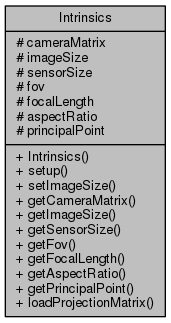
\includegraphics[width=0.3\textwidth]{class_intrinsics__coll__graph.png}
%  \caption{Clase Intrinsics}
%  \label{fig:classIntrinsics}
%\end{figure}
La clase \texttt{Intrinsics} almacena la geometría y las características internas de la cámara. La matriz intrínseca o matriz de la cámara se representa como un objeto matriz \texttt{cv::Mat} de dimensiones 3x3 formada por los siguientes parámetros:

\begin{equation}
cameraMatrix=
\begin{bmatrix}
f_{x} & \gamma & c_{x} \\
0    & f_{y}   & c_{y} \\
0    & 0      & 1
\end{bmatrix}
\end{equation}

Los parámetros $f_{x}$ y $f_{y}$ representan la distancia focal en términos de distancia. $\gamma$ representa el coeficiente de asimetría entre los ejes $X$ e $Y$, pero por simplificar el modelo, tomaremos que tiene valor 0. Finalmente, $c_{x}$ y $c_{y}$ representan las coordenadas en píxeles del punto principal, que sería idealmente en el centro de la imagen.

A partir de la matriz de la cámara y el tamaño de la imagen capturada, la clase \texttt{Intrisics} calcula el resto de parámetros propios como son el campo visual \texttt{(fov)}, la distancia focal \texttt{(focalLength)}, el centro óptico \texttt{(principalPoint)} y la relación de aspecto \texttt{(aspectRatio)} mediante la función \texttt{cv::calibrationMatrixValues}. 

\begin{listing}[
  float=ht,
  language = C++,
  caption  = {Atributos de la clase Intrinsics},
  label    = code:Intrinsics]
 cv::Mat cameraMatrix;       // (fx 0 cx, 0 fy cy, 0 0 1)
 cv::Size imageSize;         // Size of the image
 cv::Size sensorSize;        // Size of the image
 cv::Point2d fov;            // Field of view
 double focalLength;         // Focal length
 double aspectRatio;         // Aspect Ratio
 cv::Point2d principalPoint; // Principal point (center)
\end{listing}

OpenGL asume que no existe distorsión en la cámara por lo que a la hora de calcular la matriz de proyección debemos tener en cuenta que los parámetros de la matriz de la cámara deben estar corregidos. De esta forma, se utilizaran dos instancias de la clase \texttt{Instrinsics}: \texttt{distortedIntrinsics} y \texttt{undistortedIntrinsics}. La primera instancia almacena los parámetros ``reales'' mientras que en \texttt{undistortedIntrinsics} se encuentran los parámetros corregidos mediante las funciones \texttt{cv::getOptimalNewCameraMatrix} y \texttt{cv::initUndistortRectifyMap}.

\begin{listing}[
  float=ht,
  language = C++,
  caption  = {Atributos de la clase Calibration},
  label    = code:Calibration]
  //Intrinsics
  Intrinsics distortedIntrinsics;
  Intrinsics undistortedIntrinsics;
  cv::Mat distCoeffs;
  
  // Calibration parameters
  vector<vector<cv::Point2f> > imagePoints;
  vector<vector<cv::Point3f> > objectPoints;
  float reprojectionError;
  vector<float> perViewErrors;
  vector<cv::Mat> boardRotations;
  vector<cv::Mat> boardTranslations;

  // Pattern Configuration
  CalibrationPattern patternType;
  cv::Size patternSize;
  cv::Size addedImageSize;
  cv::Size subpixelSize;
  float squareSize;
 
  // Auxiliar calibration variables
  cv::Mat grayMat;
  bool fillFrame;
  cv::Mat undistortBuffer;
  cv::Mat undistortMapX, undistortMapY;
  bool ready;
 \end{listing}

Aunque el proceso de calibrado para la cámara y el proyector sigue el mismo enfoque, hay ciertas particularidades propias de cada dispositivo en el proceso de calibrado. La clase \texttt{Calibration} implementa toda la funcionalidad común, que es la mayoría, mientras que se han definido las clases \texttt{CameraCalibration} y \texttt{ProjectorCalibration} que heredan de \texttt{Calibration} y terminan de definir los procesos específicos.

Finalmente la clase \texttt{CameraProjectorCalibration} encapsula un objeto de  \texttt{CameraCalibration} y otro de \texttt{ProjectorCalibration} con los parámetros intrínsecos de ambos dispositivos e incluye los vectores de rotación \texttt{(rotCamToProj)} y traslación \texttt{(transCamToProj)} que definen las transformaciones necesarias entre el sistema de referencia de la cámara y el sistema de referencia del proyector. 

\texttt{CalibrationCore} es la encargada de inicializar la calibración de calibrado mediante la configuración establecida y define el proceso a realizar en cada una de las fases que lo compone.  bucle Update/draw

La configuración del proceso:
\begin{listing}[
  float=ht,
  language = C++,
  caption  = {Configuración de la clase CalibrationCore},
  label    = code:CalibCore]
  // Threshold parameters
  circleDetectionThreshold = 160;
  
  // Application
  diffMinBetweenFrames = 4.0; 
  timeMinBetweenCaptures = 2.0; 
  
  //Boards parameters
  numBoardsFinalCamera = 20;  
  numBoardsFinalProjector = 20;
  numBoardsBeforeCleaning = 3;  
  numBoardsBeforeDynamicProjection = 5; 
  maxReprojErrorCamera = 0.20;
  maxReprojErrorProjectorStatic = 0.25;
  maxReprojErrorProjectorDynamic = 0.43;

  // Image Size
  projectorFrame.create(cv::Size(800,600), CV_8UC1);
  
  // --- INITIAL MODE ---
  setState(CAMERA); //CAMERA, PROJECTOR_STATIC, DEMO_AR
\end{listing}
  
\subsection{Calibración de la cámara}
En esta primera fase el objetivo es obtener los parámetros intrínsecos de la cámara. De forma continua, el sistema realiza capturas de imagen. Durante este proceso, se debe mostrar a la cámara el patrón impreso en distintas posiciones y orientaciones. 

Para cada imagen capturada, se realiza el siguiente proceso:

\begin{itemize}

\item Se realiza una \textbf{búsqueda de las esquinas de los cuadrados del patrón de calibración} en la imagen. Para detectar las esquinas se utiliza la función \texttt{cv::findChessboardCorners}. A esta función se le debe proporcionar la imagen actual donde buscar el patrón, las dimensiones del patrón y un vector de \texttt{cv::Point2f} donde se almacenaran los puntos de la imagen de las esquinas detectadas. Adicionalmente, para mejorar esta detección se emplea \texttt{cv::cornerSubPix}, que se encargará de ubicar estas esquinas en medidas de subpíxeles. Si se ha encontrado el tablero de ajedrez en la imagen, el vector de puntos devuelto se guardan en el vector \texttt{imagePoints} junto con las extracciones de los frames anteriores.  

\begin{listing}[
  float=ht,
  language = C++,
  caption  = {Detección de las esquinas del patrón \emph{Chessboard}},
  label    = code:findChessBoard]
  cout << "Detecting chessboard ...";
  found = cv::findChessboardCorners(currentFrame, patternSize, pointBuf, chessFlags);

  // improve corner accuracy
  if(found) {
    if(currentFrame.type() != CV_8UC1) 
    cv::cvtColor(currentFrame, grayMat, CV_RGB2GRAY);
    else 
    grayMat = currentFrame;
    
    if(refine)
    // the 11x11 dictates the smallest image space square size allowed
    // in other words, if your smallest square is 11x11 pixels, then set this to 11x11
    cv::cornerSubPix(grayMat, pointBuf, subpixelSize,  cv::Size(-1,-1), cv::TermCriteria(CV_TERMCRIT_EPS + CV_TERMCRIT_ITER, 30, 0.1 ));
  }
  
  imagePoints.push_back(pointBuf);
\end{listing}

\item \textbf{Se generan los puntos de las esquinas del patrón en el sistema de coordenadas globales} \texttt{(objectPoints)} correspondientes a la imagen actual, en funcion del tipo, dimensiones y el valor de la medida real del lado del cuadrado del patrón que se ha impreso a través de la función \texttt{updateObjectPoints}.
\begin{listing}[
  float=ht,
  language = C++,
  caption  = {Función \texttt{Calibration::updateObjectPoints()}},
  label    = code:updateObjectPoints]
  void Calibration::updateObjectPoints() {
    vector<cv::Point3f> points = createObjectPoints(patternSize, squareSize, patternType);
    objectPoints.resize(imagePoints.size(), points);
  }
\end{listing}

\item Para \textbf{realizar la asociación entre los puntos de la imagen y los del objeto} se utiliza la funcion \texttt{cv::calibrateCamera} que estima los parámetros intrínsecos y extrínsecos de la cámara para cada una de las vistas. Recibe los \texttt{objectPoints} y los \texttt{imagePoints } de todas las capturas que llevamos realizadas y el tamaño de la imagen capturada \texttt{(addedImageSize)}, y devuelve la matriz de la cámara \texttt{(cameraMatrix)}, los coeficientes de distorsión \texttt{(distCoeffs)} y un vector con los vectores de rotación \texttt{boardRotations} y traslación \texttt{boardTranslations} que se ha estimado para cada vista del patrón. Es decir, cada rotación del vector k-ésimo junto con el vector correspondiente k-ésimo de la traslación, convierte los puntos del patrón de calibración desde el sistema de coordenadas globales (en el que se especifican los puntos del objeto) al sistema de referencia de la cámara en la vista k-ésima. La función devuelve también el error de reproyección cometido para cada una de las vistas.

\begin{listing}[
  float=ht,
  language = C++,
  caption  = {Calibrado de la cámara mediante \texttt{cv::calibrateCamera} },
   label    = code:calibrateCamera]
   cv::Mat cameraMatrix = cv::Mat::eye(3, 3, CV_64F);
   distCoeffs = cv::Mat::zeros(8, 1, CV_64F);
   int calibFlags = 0;
   float rms = cv::calibrateCamera(objectPoints, imagePoints, addedImageSize, cameraMatrix, distCoeffs, boardRotations, boardTranslations, calibFlags);
   cout << "RMS reprojection error: " << rms << endl;
 \end{listing}

\item La función \texttt{cv::checkRange} \textbf{comprueba la integridad de los elementos de la matriz de la cámara y de los coeficientes de distorsión}, asegurando que son valores numéricos válidos. 

\item A partir de los parámetros intrínsecos obtenidos, se \textbf{actualiza el error de reproyección general} de la calibración \texttt{(updateReprojectionError())}, y se \textbf{calcula la matriz de proyección de la cámara corregida} \texttt{(undistortedIntrinsics)} aplicando los valores de distorsión.
  
\item Cada cierto número de iteraciones \textbf{se eliminan las calibraciones que tienen un error de reproyección mayor que el umbral definido} en la variable \texttt{maxReprojErrorCamera}
      
\begin{listing}[
  float=ht,
  language = C++,
  caption  = {Limpieza de calibraciones},
  label    = code:clean]  
void Calibration::clean(float maxReprojErrorCamera) {
  cout << "Cleaning ...";
   int removed = 0;
   for(int i = size() - 1; i >= 0; i--) {
     if(getReprojectionError(i) > maxReprojErrorCamera) {
       objectPoints.erase(objectPoints.begin() + i);
       imagePoints.erase(imagePoints.begin() + i);
       removed++;
     }
   }
   cout << "Done!" << endl;
   if(size() > 0 && removed > 0) 
   calibrate();
}
\end{listing}
 


\end{itemize}
      
Alcanzado el número de calibraciones correctas por debajo del error definido, se procede al \textbf{almacenamiento de los últimos parámetros calculados} en un fichero de tipo YAML. Para ello se usa un objeto de tipo \texttt{cv::FileStorage} para escribir el fichero \texttt{calibrationCamera.yml} con la estructura y formato definido.

\begin{listing}[
  float=ht,
  language = C++,
  caption  = {Almacenamiento de los parámetros intrínsecos en un fichero YAML},
  label    = code:FileStorage]
  void Calibration::save(string filename, bool absolute) const {
    if(!ready){
      cout << "Calibration::save() failed, because your calibration isn't ready yet!"<< endl;
    }
    cv::FileStorage fs(filename, cv::FileStorage::WRITE);
    cv::Size imageSize = distortedIntrinsics.getImageSize();
    cv::Size sensorSize = distortedIntrinsics.getSensorSize();
    cv::Mat cameraMatrix = distortedIntrinsics.getCameraMatrix();
    fs << "cameraMatrix" << cameraMatrix;
    fs << "imageSize_width" << imageSize.width;
    fs << "imageSize_height" << imageSize.height;
    fs << "sensorSize_width" << sensorSize.width;
    fs << "sensorSize_height" << sensorSize.height;
    fs << "distCoeffs" << distCoeffs;
    fs << "reprojectionError" << reprojectionError;
    fs << "features" << "[";
    for(int i = 0; i < (int)imagePoints.size(); i++) {
      fs << "[" << imagePoints[i] << "]";
    }
    fs << "]";
  }
\end{listing}

Una vez finalizada la calibración de la cámara, el sistema continua para obtener los parámetros intrínsecos del proyector.

\subsection{Calibración del proyector}
El cálculo de los parámetros intrínsecos de proyector se realiza mediante el mismo enfoque que en la cámara. Considerándolo como una \textit{«cámara inversa»} se puede aplicar el mismo modelo matemático de cámara \emph{pinhole}.

En esta fase, el sistema proyecta continuamente un patrón de círculos asimétricos con un tamaño y en una posición fija. El objetivo es que la cámara detecte el patrón y pueda establecer, una primera aproximación de la matriz de proyección del proyector. Posteriormente, estos parámetros serán refinados en la siguiente fase del proceso de calibrado, mediante la proyección del patrón dinámicamente.

En primer lugar, Se carga el fichero con los parámetros intrínsecos de la cámara y se establecen los puntos del patrón asimétrico en la imagen que se va a proyectar \texttt{(imagePoints)} y en el sistema de referencia global \texttt{(objectPoints)} utilizando parámetros y distancias fijas.  

\begin{listing}[
  float=ht,
  language = C++,
  caption  = {Inicialización de la fase de calibrado del proyector},
  label    = code:ProjectorStatic]
calibrationCamera.load("calibrationCamera.yml",false);
camProjCalib.resetBoards();
calibrationCamera.setupCandidateObjectPoints();
calibrationProjector.setStaticCandidateImagePoints();
\end{listing}

Se busca el patrón asimétrico en la imagen capturada, para ello se utiliza la funcion \texttt{cv::findCirclesGrid} que intenta determinar si la imagen de entrada contiene una cuadrícula de círculos. Si es así, la función localiza los centros de los círculos. Para la detección de los círculos esta función se apoya en un detector de regiones \emph{(Blob detector)} que configuramos mediante los siguiente parámetros para adaptar la búsqueda en función del tamaño de la imagen y el tamaño de las regiones que se van a detectar.

\begin{listing}[
  float=ht,
  language = C++,
  caption  = {Parametrización del \emph{Blob Detector}},
  label    = code:BlobDetector]
cv::SimpleBlobDetector::Params params;
params.minArea = 10;
params.minDistBetweenBlobs = 5;
cv::Ptr<cv::FeatureDetector> blobDetector = new cv::SimpleBlobDetector(params);
bool bProjectedPatternFound = cv::findCirclesGrid(processedImg, calibrationProjector.getPatternSize(), circlesImgPts, cv::CALIB_CB_ASYMMETRIC_GRID | cv::CALIB_CB_CLUSTERING, blobDetector);
\end{listing}

Se aplica una binarización de la imagen de entrada que permite la segmentación de los círculos proyectados y realizar una separación del patrón de tablero de ajedrez.

  
Encontrado el patrón de círculos, obtenemos los vectores de rotación \texttt{boardRot} y translación \texttt{boardTrans} de los puntos proyectados en el sistema de referencia de la cámara mediante la funcion \texttt{cv:solvePnP}


 Transform all image points to world points in camera reference frame  and then into the plane reference frame
Se transforman los punto de la imagen a puntos reales en el sistema de referencia de la cámara, y después al sistema de referencia del patrón
La cámara se utiliza para calcular la posición 3D de los círculos proyectados (por retroproyección) según el  sistema de coordenadas local de la cámara, y luego en el sistema de coordenadas local del patrón (que es el sistema de coordenadas "mundo"). Esto se hace en el método de "backProject" (método de la calibración clase, pero llama sólo cuando el objeto es de tipo "cámara"). 

Esto significa que podemos comenzar a computar los instrinsics del proyector porque tiene puntos 3d (los círculos proyectados) en coordenadas del mundo, y sus respectivos "proyección" "imagen" en el proyector plano. 

Para realizar la asociación entre los puntos de la imagen y los del objeto se utiliza la funcion \texttt{cv::calibrateCamera} que estima los parámetros intrínsecos y extrínsecos de la cámara para cada una de las vistas. Recibe los objectPoints y los imagePoints de todas las capturas que llevamos realizadas y el tamaño de la imagen \texttt{addedImageSize}. y devuelve la matriz de la cámara \texttt{cameraMatrix}, los coeficientes de distorsión {distCoeffs} y un vector con los vectores de rotación y traslación que se ha estimado para cada vista del patrón. Las funciones checkRange comprobar que cada elemento de la matriz de la cámara y de los coeficientes de distorsión es ni NaN ni infinito. Actualización de distortedIntrinsics, actualización del error de reproyección y calculo de undistortedIntrinsics:distortedIntrinsics.setup(cameraMatrix, addedImageSize);  updateReprojectionError();   updateUndistortion();

calibrationProjector.calibrate();

Se comprueba que el error de reproyección no es superior al umbral definido.

Este proceso se repite hasta capturar un número de patrones definido en la configuración. Una vez alcanzado el numero de patrones capturados y con un error inferior al umbral pasamos a la siguiente fase de calibrado.

\subsection{Calibración del sistema estéreo cámara-proyector}
En esta fase refinaremos la calibración de los parámetros intrínsecos del proyector calculados en la fase previa y realizaremos los cálculos para obtener los parámetros extrínsecos del sistema estéreo cámara-proyector.

A partir de ahora, generamos el patrón de círculos asimétricos de manera dinámica. A partir de la posición y las dimensiones del patrón de tablero de ajedrez observado por la cámara, con la función \texttt{setDynamicProjectorImagePoints} se calcula y genera un patrón de círculos asimétricos que se proyectará junto al de ajedrez. 

Dispondremos entonces de los puntos 3D en el sistema de referencia global (el patrón), que son los círculos proyectados, y también su proyección (puntos 2D en la imagen) en el sistema de referencia de la cámara y en el sistema de referencia del proyector. Esto significa que se puede utilizar  un procedimiento de calibración estéreo como el que proporciona OpenCV. 


Consideraremos en nuestro sistema estéreo que la posición y orientación relativa entre la cámara y el proyector es fija. En los paso previos, se ha  calculado la pose de un objeto respecto a la cámara $(R_1, T_1)$ y la pose para el mismo objeto pero respecto al proyector $(R_2, T_2)$, entonces esas poses se relacionan entre sí. Esto significa que, dado $(R_1,T_1)$, es posible calcular $(R_2,T_2)$ conociendo la posición y orientación de la segunda cámara con respecto a la primera cámara. Esto es lo que hace la función descrita. Calcula $(R,T)$ de modo que:

\begin{equation}
R_2 = R * R_1
T_2 = R * T_1 + T,
\end{equation}

Opcionalmente, se calcula la matriz esencial $E$:
\begin{equation}
E=\begin{bmatrix}
0 & -T_2 & -T_1\\ 
T_2 & 0  & -T_0\\ 
-T_1 & T_0 & 0 
\end{bmatrix} * R
\end{equation}

donde $t_i$ son componentes del vector de traslación $T: T = [T_0, T_1, T_2] ^ T$. Y la función también puede calcular la matriz $F$ fundamental:
\begin{equation}
F = cameraMatrix_2^ {-T} * E * cameraMatrix_1^{-1}
\end{equation}


Mediante la función \texttt{cv::stereoCalibrate} se estima la matriz de transformación entre dos cámaras que formen un par estéreo. En nuestro caso la cámara y el proyector. 

La funcion \texttt{cv::stereoCalibrate} también permite obtener los parámetros intrínsecos de cada dispositivo, sin embargo debido a la alta dimensionalidad del espacio de parámetros y el ruido que pueden introducir las imágenes de entrada, la funcion puede divergir de la solución correcta. Por tanto utilizaremos los parámetros intrínsecos calculados en las fases previas para cada uno de los dispositivos de forma individual, proporcionándolos a la funcion e indicándolo mediante el \emph{flag} CV\_CALIB\_FIX\_INTRINSIC. Esto acción, simplifica los cálculos que tiene que realizar la función y que se realicen cálculos erróneos de unas matrices de proyección que ya se han obtenido previamente con bastante precisión. 

Como hemos indicado, debemos proporcionar los puntos del patrón de calibración y las proyecciones de estos puntos observados respecto a la cámara y el proyector. \texttt{setDynamicProjectorImagePoints()} nos genera los puntos del patrón asimétrico y almacena la proyección de los puntos respecto de la cámara. La funcion \texttt{calibrationProjector.calibrate()} obtiene los parámetros intrínsecos y la proyección de los puntos del patrón respecto del proyector. 

Al estar diseñado el bucle del programa mediante un enfoque \emph{update/draw}, tenemos que proceder en dos iteraciones para dar tiempo a la imagen proyectada a refrescarse antes de tratar de detectarlo. De lo contrario podemos estar detectando el viejo patrón proyectado, pero el uso de los puntos de imagen más recientes (que rompe por completo la calibración por supuesto)

Con todos los parámetros necesarios calculados:
\begin{itemize}
  \item objectPoints: Puntos del patrón generado dinámicamente.
  \item auxImagePointsCamera: Proyecciones de los puntos del patrón desde el punto de vista de la cámara
  \item calibrationProjector.imagePoints: Proyecciones de los puntos del patrón desde el punto de vista del proyector
  \item cameraMatrix: Matriz de parámetros intrínsecos de la cámara
  \item cameraDistCoeffs: Coeficientes de distorsión de la cámara
  \item projectorMatrix: Matriz de parámetros intrínsecos del proyector
  \item projectorDistCoeffs: Coeficientes de distorsión del proyector
  \item calibrationCamera.getDistortedIntrinsics().getImageSize(): Tamaño de la imagen utilizada.
\end{itemize}  
 
\texttt{cv::stereoCalibrate} devuelve la matriz de rotación \texttt{rotation3x3}, el vector de translación \texttt{transCamToProj} entre el sistema de referencia de la cámara y el proyector y el error de reproyección obtenido. La función \texttt{cv::Rodrigues} transforma la matriz de rotación en el vector de rotación \texttt{rotCamToProj} que almacena el proceso de calibrado.

Cada cierto número de iteraciones, configurable en el sistema, se eliminan las capturas del patrón que el error de reproyección supere un determinado umbral. Y finalmente al alcanzar un numero suficiente de calibraciones correctas, se toman los valores de los parámetros intrínsecos y extrínsecos del proyector a los que converge el proceso como los finales, guardándolos en un fichero de tipo YAML al igual que se realizó con los parámetros intrínsecos de la cámara mediante un objeto de tipo cv::FileStorage. calibrationProjector.yml CameraProjectorExtrinsics.xml


Para finalizar, el sistema pasa al modo de validación del proceso de calibrado, donde de manera visual, comprobaremos la precisión de la calibración realizada.
  %setState(DEMO_AR);

\subsection{Verificación del proceso de calibrado}
Carga de los ficheros YAML y obtener instancias de los objetos:
%CameraCalibration calibrationCamera = camProjCalib.getCalibrationCamera();
%ProjectorCalibration calibrationProjector  = camProjCalib.getCalibrationProjector();

Se busca el patrón de tablero de ajedrez en la imagen y se extraen los puntos de las esquinas \texttt{chessImgPts}
%bool bPrintedPatternFound = calibrationCamera.findBoard(cameraFrame, chessImgPts, true);

Calcula los vectores de rotación \texttt{cv::Mat boardRot} y traslación \texttt{cv::Mat boardTrans} del patrón a la cámara
%calibrationCamera.computeCandidateBoardPose(chessImgPts, boardRot, boardTrans);

Seleccionamos los ObjectPoints correspondientes a las cuatro esquinas del patrón y se almacenan en \texttt{vector<cv::Point3f> auxObjectPoints}

%cv::Mat rotObjToProj, transObjToProj;

Componemos los vectores de rotación y traslación del objeto a la cámara con vectores cámara al projector para obtener las transformaciones objeto a proyector
%cv::composeRT(boardRot,  boardTrans,
%camProjCalib.getCamToProjRotation(), camProjCalib.getCamToProjTranslation(),
%rotObjToProj, transObjToProj);

Proyectamos con la funcion \texttt{cv::projectPoints} los puntos de las cuatro esquinas del patrón \texttt{auxObjectPoints}, mediante las transformaciones objeto-proyector y los parámetros intrínsecos del proyector

%projectPoints(cv::Mat(auxObjectPoints),
%rotObjToProj, transObjToProj,
%calibrationProjector.getDistortedIntrinsics().getCameraMatrix(),
%calibrationProjector.getDistCoeffs(),
%out);

Establecemos los puntos obtenidos en la proyección \texttt{vector<cv::Point2f> out} como la salida que tiene que representar el proyector y que deben coincidir físicamente si se ha realizado una buena calibración. calibrationProjector.setCandidateImagePoints(out);


\section{Tracking y registro}
El cálculo del registro requiere posicionar el sistema cámara-proyector, mediante su posición y
rotación, relativo a las hojas de papel que se encuentren en la escena capturada. Los métodos de
tracking, en general, son los encargados de obtener una estimación de la trayectoria que realiza un
objeto.

En GrayAR, se ha optado por implementar un sistema de tracking visual basado en una aproximación \textbf{\textit{bottom-up}}\cite{Marimon}, en la que se calculan los seis grados de libertad de la cámara a partir de lo que se está
percibiendo en la imagen.

%\begin{itemize}
%\item Una primera fase basada en una aproximación \textbf{\textit{bottom-up}}\cite{Marimon}, en la que se
%  calculan los seis grados de libertad de la cámara (ver sección Pose) a partir de lo que se está
%  percibiendo en la imagen.

%  \item En el caso de no poder determinar la \emph{pose} en la fase anterior, se realiza un enfoque
%  \textbf{\textit{top-down}}\cite{Marimon}, que estima la posición y rotación del papel en función de las
%  observaciones almacenadas en los estados anteriores.
%\end{itemize}


Conociendo las posiciones 2D de las aristas y vértices que definen la hoja de papel, y el modelo de
proyección de la cámara es posible estimar la posición y rotación 3D de la cámara relativamente al
documento. Aprovechando que conocemos la estructura de formato normalizado (según ISO 120/DIN 476) de una
hoja de papel, con un tamaño previamente conocido nos permite definir un sistema de coordenadas
local de cada hoja detectada, de modo que obtengamos la matriz de transformación 4x4 del sistema de
coordenadas de la hoja al sistema de coordenadas de la cámara.

El enfoque utilizado es similar al de ArUCo y ARToolkit, mediante un algoritmo de detección de bordes y un
método de estimación de la orientación. Sobre la imagen obtenida se inicia el primer paso de búsqueda de hojas de
papel. La imagen se convierte a blanco y negro para facilitar la detección de cuadriláteros;
primero se convierte a escala de grises, y después se binariza eligiendo un parámetro de
umbral “threshold” que elige a partir de qué valor de gris (de entre 256 valores distintos) se
considera blanco o negro. A continuación el algoritmo de visión por computador
extrae componentes conectados de la imagen previamente binarizada,cuya área es
suficientemente grande como para ser una hoja de papel. A estas regiones se les aplica un algoritmo
de detección de contornos, obteniendo a continuación los vértices y aristas que definen la
región de la hoja en 2D.

\subsection{Conversión a escala de grises (Grayscale)}
El primer paso en el proceso de detección consiste en convertir el frame capturado por la cámara a
escala de grises mediante la función \texttt{cv::cvtColor}. Esta función convierte una imagen de un
espacio de color a otro. La constante \texttt{CV\_BGR2GRAY} sirve para indicar que queremos pasar de
una imagen BGR (estándar de OpenCV) a otra en escala de grises.

\subsection{Umbralización o binarización (Thresholding)}
La umbralización consiste en definir un valor umbral y compararlo con cada uno de los píxeles de la
imagen. A los píxeles que estén por debajo del umbral se les asigna un valor, y a los que estén por
encima otro. De esta forma se divide toda la población de valores en tan sólo dos grupos, reduciendo
considerablemente la complejidad de la información a analizar.

En ARgos, se han desarrollado tres soluciones distintas para tratar de resolver este problema del
thresholding básico (fijo, adaptativo y el método Canny). En un principio, solo se implementaron
los métodos fijos y adaptativo, pero en una fase de optimización realizada posteriormente, se incluyo
el método Canny. Este algoritmo proporcionaba bordes más precisos, y es  tolerante a las
variaciones de iluminación, produciendo menores índices de ruido en la imagen binarizada.

\subsection{Extracción de contornos}
El siguiente paso del proceso es la detección de contornos, una operación un tanto distinta a las
anteriores por dos motivos principales. El primero es que no consiste en iterar aplicando una misma
función de forma monótona sobre todos los píxeles de la imagen. Y el segundo, es que el resultado que
se obtiene no es una nueva imagen, sino un colección de conjuntos de puntos sobre la imagen.

Para este paso se parte de la imagen resultante del paso anterior. Es decir, de una imagen que tan
solo consta de píxeles con valor cero o uno. Sobre ella se aplica un algoritmo que la barre,
empezando por su esquina superior izquierda, a la busca de un primer píxel a uno, y que cuando lo
encuentra es capaz de seguir la cadena de píxeles con valor uno que se encuentran unidos a él hasta
volver al píxel de partida. Esa cadena de píxeles a uno encontrados se denomina contorno. Y es más,
el algoritmo es capaz de encontrar todos los contornos presentes en la imagen, ya que cuando termina
con uno empieza de nuevo el proceso hasta asegurarse de haber barrido la imagen por completo.

El algoritmo es bastante potente, ya que no sólo es capaz de encontrar los contornos exteriores,
sino también los interiores a otros, y retornarlos clasificados jerárquicamente. ARgos utiliza la
función \texttt{cv::findContours} que implementa este algoritmo. En la documentación, así como la
referencia de implementación, se refiere al \textit{paper} original «Topological structural analysis
of digitized binary images by border following» de Satoshi Suzuki and Keiichi Abe.

Básicamente hay un contador de contornos encontrados y un buffer de píxeles recorridos. El contador
se inicializa a cero y el buffer con una copia de la imagen original. Se barre el buffer de arriba
abajo y de izquierda a derecha. Una transición de un píxel 0 a otro 1 indica que se ha detectado un
borde exterior, momento en que se suma uno al contador de contornos encontrados y se buscan todos
los píxeles 1 vecinos del encontrado. Si el píxel no tiene vecinos a 1 se cambia el valor del píxel
por el del contador con signo contrario y se empieza otra vez con el siguiente píxel. En caso
contrario se cambia el valor del píxel por el del contador, excepto que su valor sea mayor que 1, lo
que significa que ya ha sido visitado, y se continúa buscando vecinos a 1 hasta retornar al píxel
inicial. Una transición de un píxel con valor igual o mayor que 1 a otro 0 indica que se ha
detectado un borde interior, momento en que se repite el mismo proceso usado para los contornos
exteriores.

El algoritmo presenta una pequeña dificultad en los bordes de la imagen, y para solventarlo
presupone que la imagen está rodeada por los cuatro lados de píxeles con valor 0. Es decir, que el
buffer que utiliza tiene una fila más por encima y por debajo, y una columna más a derecha e
izquierda, que la imagen original.


\subsection{Aproximación a polígonos (Douglas-Peucker)}
Los contornos de los que se parte para este paso son colecciones de puntos. Todos y cada uno de los
píxeles que forman parte de ellos, ya que no se guardaron sólo las esquinas, sino cada píxel
individual encontrado. Esto permite tomar algunas decisiones tempranas, como por ejemplo descartar
los contornos que no tengan un mínimo de puntos. Es decir, aquellos que no son susceptibles de formar
la hoja de papel. ARgos descarta aquellos que no tengan un área delimitada entre 47000 y 49000
píxeles.

Sobre aquellos contornos que cumplan con la restricción de superficie, se calcula la envoltura
convexa del contorno. Matemáticamente se define la envoltura convexa de un conjunto de puntos $X$ de
dimensión $n$ como la intersección de todos los conjuntos convexos que contienen a $X$.

Dados $k$ puntos $x_1, x_2,\dots x_k$ su envoltura convexa $C$ viene dada por la expresión:
\begin{equation}
C(X) =\left\{\sum_{i=1}^k \alpha_i x_i \ \Bigg | \ x_i\in X, \, \alpha_i\in \mathbb{R}, \, \alpha_i \geq 0 \, , \sum_{i=1}^k \alpha_i=1\right\}
\end{equation}

Es decir, teniendo un conjunto de puntos en el plano, su envoltura convexa está definida por el
polígono convexo de área mínima que cubre todos los puntos (esto es, todos los puntos están dentro
del polígono). OpenCV proporciona la función \texttt{cv::convexHull} para encontrar la envoltura de
una conjunto de puntos 2D utilizando el algoritmo de Sklansky con una complejidad $O(N log N)$ en su
actual implementación.

El objetivo del cálculo de la envoltura es la de obtener un contorno \emph{limpio}, ya que tras este
paso se han eliminado puntos interiores debidos a reflejos, sombras o ruido en la imagen que se hubiesen
detectado. Otra ventaja, es que permite que existan pequeños solapamientos en los bordes, y aún así, se
siga detectando el contorno del papel.

GrayAR utiliza la función \texttt{cv::approxPolyDP}  para convertir una colección de puntos en un
polígono mediante el algoritmo de Douglas-Peucker. El algoritmo admite como entrada una lista de
puntos y una distancia máxima permitida. Define un segmento que va desde el primer punto de la lista
hasta el último, y calcula la distancia más corta que hay desde dicho segmento a todos y cada uno
del resto de puntos de la lista. Si encuentra un punto a una distancia mayor que la máxima pasada
como parámetro divide la lista y el segmento en dos, utilizando el punto encontrado como nuevo
extremo. Y vuelve a empezar el proceso comprobando cada nueva lista contra cada nuevo segmento de
forma individual, creando nuevas listas y segmentos si fuera necesario, de forma recursiva.

ARgos utiliza como distancia máxima para al algoritmo el 10\% del número de puntos que tiene cada
contorno de forma individual. Una vez convertidos los puntos a polígonos se descartan los que no
tengan cuatro lados.

En este punto, en los casos en los que no existan grandes solapamientos sobre el papel, debemos
obtener una serie de polígonos que se corresponden con las hojas detectadas en la imagen.

\subsection{Búsqueda de cuadriláteros en el espacio de Hough}
Mientras se este realizando alguna interacción con el documento, nuestra mano, dedos e incluso parte
del brazo estarán solapando gran parte de la hoja que queremos detectar. Tras aplicar el detector de
bordes a la imagen recibida, obtenemos segmentos no conectados que las funciones anteriores no serán
capaces de clasificar como cuadriláteros candidatos a ser una hoja de papel.

En estos casos, la búsqueda de la hoja de papel en la imagen se realiza mediante detectores de líneas basados
en la transformada de Hough.

La transformada de Hough es una técnica para detectar bordes llevando los puntos al espacio
paramétrico donde se transforman en rectas.
Basándose en lo anterior, la recta $y = m*x+n$ se puede representar como un punto $(m,n)$ en el
espacio de parámetros. Sin embargo, cuando se tienen rectas
verticales, los parámetros de la recta $(m,n)$  no están definidos. Por esta razón se utilizan los parámetros
que describen una recta en coordenada polares, denotados $(\rho,\theta)$.

El parámetro $\rho$ representa la distancia entre el origen de coordenadas y el punto$(x,y)$,
mientras que $\theta$ es el ángulo del vector director de la recta perpendicular a la recta original
y que pasa por el origen de coordenadas.

Usando esta parametrización, la ecuación de una recta se puede escribir de la siguiente forma:

\begin{equation}
y=(-\dfrac{\cos \theta}{\sin \theta}) * x + (\dfrac{\rho}{\sin \theta})
\end{equation}
que se puede reescribir como
\begin{equation}
\rho=x * \cos \theta + y * \sin \theta
\end{equation}

Entonces, es posible asociar a cada recta un par $(\rho,\theta)$ que es único si $\theta \in
[0,\pi)$ y $\rho \in \mathbb{R}$ ó $\theta \in [0,2\pi)$ y $\rho \geq 0$. El espacio
$(\rho,\theta)$ se denomina espacio de Hough para el conjunto de rectas en dos dimensiones.

Para un punto arbitrario en la imagen con coordenadas $(x_0,y_0)$, las rectas que pasan por ese punto
son los pares  $(\rho,\theta)$ con  $\rho=x*\cos \theta + y * \sin \theta$ donde $\rho$ (la
distancia entre la línea y el origen) está determinado por $\theta$. Esto corresponde a una curva
sinusoidal en el espacio  $(\rho,\theta)$, que es única para ese punto. Si las curvas
correspondientes  a dos puntos se intersecan, el punto de intersección en el espacio de Hough
corresponde  a una línea en el espacio de la imagen que pasa por estos dos puntos. Generalizando, un
conjunto de puntos que forman una recta, producirán sinusoides que se intersecan en los parámetros
de esa línea. Por tanto, el problema de detectar puntos colineales se puede convertir en un problema
de buscar curvas concurrentes.

Las zonas de este espacio donde más líneas se cortan se convierten en parámetros de posibles rectas
en el espacio de la imagen.

Se seleccionan un conjunto de las rectas detectadas para ser examinado en función de las siguientes características:

\begin{itemize}
\item El segmento se encuentra dentro o en la proximidades de la zona de proyección del
  sistema. Con esta restricción descartaremos aquellos segmentos que sabemos de antemano que no van
  a ser hojas de papel, como por ejemplo, otros objetos que se encuentren en la imagen o los bordes
  de la superficie donde se encuentra en prototipo.
\item El segmento es mayor que un valor umbral.
\item Sólo se tienen en cuenta los segmentos más próximos a los límites de proyección. El detector
  de Hough puede encontrar rectas en el interior de la hoja de papel que estamos buscando. Así solo
  seleccionaremos los posibles candidatos a formar el borde del papel.
\item Los ángulos que formen dos rectas contiguas estará comprendido dentro del rango de 75º a 105º.
\item Los ángulos que formen dos rectas opuestas deben ser cercanos a 180º ó 360º.
\end{itemize}

Tras la selección anterior obtendremos un conjunto de segmentos de rectas extraídas de la
imagen. Cuatro segmentos se consideran que formarán un cuadrilátero candidato si cumplen los
siguientes criterios:
\begin{itemize}
\item Las intersecciones de los cuatro segmentos están dentro de la imagen y próximos a la zona de
  proyección.
\item Sólo intersecan en cuatro puntos.
\item El área del cuadrilátero delimitado por las intersecciones esta entre 47000 y 49000 píxeles,
  ya que garantiza que el cuadrilátero que se detectó representa una hoja de papel.
\end{itemize}

Para ello se generan las posibles combinaciones de 4 segmentos del conjunto de rectas detectadas y
se analizan los criterios anteriores.

\subsection{Filtrado final}
Aún realizando todos estos descartes, ARgos incorpora un control adicional, ya que debido a que en
los pasos previos se detectan contornos tanto exteriores como interiores, puede ocurrir que se
detecten dos cuadriláteros, uno dentro de otro, siendo necesario descartar el más interno.
ARgos calcula la distancia media entre las esquinas de los polígonos y si encuentra dos que están
muy cerca descarta el de menor perímetro, que necesariamente será el más interno.

Por último, para el cálculo de las distancias entre esquinas es necesario un paso previo
en el que las esquinas tienen que estar ordenadas en el sentido contrario de las agujas del reloj
\textit{(anti-clockwise order)}.

\subsection{Cálculo de parámetros extrínsecos de la cámara}
Una vez detectadas e identificadas las hojas de papel de la imagen, se procede a calcular los parámetros extrínsecos de la cámara respecto a cada una de ellas. Para la mayoría de los cálculos basta con considerar a la lente como un agujero puntual a través del que pasa la luz a través de un centro de proyección común.

Essential problem in AR: POSE ESTIMATION
WHERE to put the CG object
ORIENTAION of CG object
SIZE of CG object

(translation)
(rotation)
(scaling)

Supongamos que se visualiza un objeto que se encuentra a una distancia $x_{1}$ de la lente, y que la
imagen proyectada por los rayos que salen de la lente se forma a una distancia $x_{2}$ tras la
lente. Se denomina disstancia focal a la relación que existe entre $x_{1}$ y $x_{2}$ :
\begin{equation}
\dfrac{1}{f} = \dfrac{1}{x_{1}} + \dfrac{1}{x_{2}}
\end{equation}

A la hora de representar los objetos del espacio observado (3D), se convierten a un plano de
visión (2D), y se tendrá que definir cual es la correspondencia entre las coordenadas del espacio y las de la representación. Para facilitar esta conversión, se utiliza el sistema de coordenadas \emph{«homogéneo»}. Este sistema de coordenadas tiene la particularidad de que permite pasar fácilmente coordenadas de un número de dimensiones a otro. Para ello, almacena las coordenadas con una dimensión adicional, de tal forma que para un espacio de 3D, utilizaríamos 4 coordenadas. El valor de la coordenada adicional indica entre otras cosas, si el punto se encuentra en el infinito, valor 0, o es un punto cualquiera, valor distinto de 0. En este sistema, si dos coordenadas son proporcionales, se refieren al mismo punto.

Las matrices de transformación, utilizadas para pasar de unas dimensiones a otras, suelen incluir 3 tipos de transformaciones: Rotación, Translación y eScalado. Podemos representarlas así:
\begin{equation}
  [R|t] = \begin{bmatrix} SR_{1,1} & SR_{1,2} & SR_{1,3} & T_{1}  \\
                          SR_{2,1} & SR_{2,2} & SR_{2,3} & T_{2}  \\
                          SR_{3,1} & SR_{3,2} & SR_{3,3} & T_{3}  \\
                             0    &     0    &     0    &  1
  \end{bmatrix}
\end{equation}

Para convertir las coordenadas del mundo a coordenadas de pantalla, de espacio tridimensional a bidimensional, los sistemas de visión artificial utilizan la siguiente fórmula:

\begin{equation}
q=MQ
\end{equation}
donde
\begin{equation}
  q=\begin{bmatrix} x \\ y \\ z \end{bmatrix} \quad M=\begin{bmatrix} f_{x} & 0 & c_{x} \\ 0 & f_{y} & c_{y} \\ 0 & 0 & 1 \end{bmatrix} \quad Q=\begin{bmatrix} X \\ Y \\ Z \end{bmatrix}
\end{equation}

Por tanto, $q$ representa el espacio bidimensional en coordenadas homogéneas, y $Q$ el espacio
tridimensional. $f_{x}$ es la distancia focal en el eje $X$, $f_{y}$ la distancia focal en el eje
$Y$, ($c_{x},c_{y}$) marcan el punto principal, el punto donde el eje de visión corta el plano de
visión (normalmente suele estar en el centro de la imagen, o muy cerca).

En ARgos se utiliza la función de OpenCV \texttt{cv::solvePnp}. Está, calcula la \emph{pose} (rotación y
traslación) de la hoja de papel, dado un conjunto de puntos del objeto \texttt{(ObjPoints)}, sus proyecciones en
la imagen correspondiente \texttt{(ImagePoints)}, así como la matriz de la cámara \texttt{(camMatrix)} y los coeficientes
de distorsión \texttt{(distCoeff)}. Esta función encuentra una \emph{pose} que minimiza el error de reproyección, es
decir, la suma de los cuadrados de las distancias entre las proyecciones \texttt{imagePoints} observados y
los \texttt{objectPoints} proyectados.

Se establece el centro del papel como centro de coordenadas $(0,0,0)$, por lo que las esquinas que se le proporcionan a la función son :
\begin{equation}
ObjPoints =\begin{bmatrix} -w/2 & -h/2 & 0 \\
                            w/2 & -h/2 & 0 \\
                            w/2 &  h/2 & 0 \\
                           -w/2 &  h/2 & 0
\end{bmatrix}
\end{equation}
Siendo $h$ y $w$ la altura y anchura de la hoja de papel respectivamente. Los ImagePoints corresponden a los píxeles que
representan las esquinas de la marca detectada, camMatrix son los parámetros intrínsecos de la
cámara y distCoeff, el vector de coeficientes de distorsión. Estos últimos parámetros se obtienen en
el proceso de calibración de la cámara y se mantienen fijos y conocidos durante todo el proceso.

\subsection{Refinamiento de la \emph{pose}}
El posicionamiento calculado puede variar en cada frame, aun cuando el papel no se haya movido
realmente. Esto puede ser debido a variaciones en la iluminación que alteran sensiblemente los
procesos de detección o errores debido a la naturaleza imprecisa de los métodos utilizados.

Este refinamiento de las percepciones se basa en la capacidad del sistema de almacenar las últimas
\textit{n} percepciones. Este parámetro es configurable en tiempo de compilación.


Cuando se recibe una última percepción, se calcula una media ponderada con las cuatro últimas
percepciones, de forma que la percepción refinada es la resultante de la siguiente fórmula:
\begin{equation}
P_{actual} = P_1*0.5 + P_2*0.25 + P_3*0.15 + P_4*0.1
\end{equation}

Siendo $P_1$ la percepción más reciente, y el resto las percepciones almacenadas en el histórico. De esta forma, se da más peso a la percepción más actual, pero se tiene en cuenta las anteriores. El resultado es un movimiento más fluido y suave, aunque da la sensación de haber un \textit{delay} al momento de representar la posición. Este retraso es lógico, al tener en cuenta percepciones pasadas.

%\subsection{Tracking mediante filtros de partículas}
%From the detection result, we have 2D positions of the four corners of the quadrangle. Since we are using a cardboard with known size, and the camera is calibrated, we can compute the relative rotation and translation of the camera to the cardboard. Then, our tracking state at frame k is represented by this relative pose in the following form
%\begin{equation}
%q_k = \left \lfloor r_x \quad r_y \quad  r_z \quad  t_x \quad  t_y \quad t_z  \right \rfloor
%\end{equation}

%Dónde $rx$, $ry$ y $rz$ son los ángulos de rotación a lo largo de los ejes $X$, $Y$, $Z$,
%respectivamente. $tx$, $ty$ y $tz$ son los ángulos traslación respectivamente a cada uno de sus ejes.

%El filtro de partículas se utiliza para estimar la densidad posterior de la pose de la cámara. La
%pose se representa como un conjunto de partículas discretas. Cada partícula tiene un peso para
%indicar el grado de confianza que representar la pose de la cámara.

%Los dos componentes principales de un filtro de partículas son el modelo dinámico del estado y el
%modelo de observación. El modelo dinámico estado determina cómo las partículas se propagan frame a
%frame. Es decir, la definición de la densidad $p(q_k|q_{k-1})$. El modelo de observación determina
%cómo se asignan pesos a las partículas que proporcionan la observación en ese marco. Que la
%observación en la trama actual sea $y_k$ y la secuencia de la observación hasta el fotograma actual
%$y_{1: k}$ , el filtro de partículas realiza el seguimiento de forma recursiva por la aproximación
%de la densidad posterior $p(q_k|y_{1:k})$. La salida del filtro de
%partículas es un conjunto de las muestras ponderadas $\left \{\left \{ q_k^1 \quad w_k^1 \right \},
%  \dots, \left \{ q_k^s \quad w_k^s  \right \}\right \}$ donde $S$ es
%el número de partículas. El diagrama de flujo del filtro de partículas utilizado en nuestro proyecto se muestra en la Figura 4.

%\subsubsection{Modelo dinámico de estado}
%Dado que la superficie cuadrangular está en movimiento libre, un modelo de paseo aleatorio simple
%basado en una densidad uniforme $U$ sobre el estado anterior [5] se utiliza. La variable e representa
%la incertidumbre sobre el movimiento del cuadrilátero detectado.

%\begin{equation}
%p(q_k|q_{k-1}) = U (q_{k-1} - e, q_{k-1} + e)
%\end{equation}

%\subsubsection{Modelo de observación}
%La observación en nuestro algoritmo es (18). Representa el mapa de características del segmento de
%línea obtenido de la trama de imagen actual.

%\begin{equation}
%y_k = L = \left \{l_1^k,l_2^k, \dots, l_m^k\right \}
%\end{equation}

%Para evaluar la probabilidad de cada partícula, lo primero que re-proyecto de las cuatro esquinas
%del cuadrilátero en el plano de la imagen de acuerdo con la postura representada por la
%partícula. Luego, se utiliza un algoritmo de coincidencia línea basado en distancias punto de línea
%y las diferencias angulares para encontrar las mejores líneas que coinciden con las cuatro líneas
%laterales del cuadrilátero en el marco actual. Entonces, si todas las líneas laterales del
%cuadrilátero representado por la partícula pueden igualar a un segmento de línea, podemos formar un
%cuadrilátero por los segmentos de línea coincidentes. Este patio se comprueba mediante los tres
%primeros criterios en el algoritmo de detección de cuadrilátero.

%Si cualquiera de las líneas laterales no pueden igualar a un segmento de línea en el mapa de entidad
%de línea o el cuadrángulo formado no puede pasar el procedimiento de comprobación, un peso muy
%pequeño se le asignará a la partícula. De lo contrario, la partícula puede igualar a un cuadrilátero
%real en la imagen actual. Para dar un resultado de seguimiento más preciso, se introdujo un esquema
%de reemplazo en nuestro modelo de observación. Para las partículas que pasan los criterios de
%coincidencia de línea y cuadrangulares procedimientos de comprobación, las cuatro líneas
%coincidentes forman un cuadrilátero real en la escena.

%A continuación, las cuatro esquinas del cuadrilátero se calculan a partir de las cuatro
%líneas. Estas esquinas entonces reemplazar los de la partícula. De esta manera, todas las partículas
%que sobreviven a partir de los procedimientos de evaluación representarán un cuadrilátero real en la
%escena. Desde las esquinas se calculan a partir de las líneas, la precisión de seguimiento puede
%estar en el nivel sub-píxel. La probabilidad se calcula entonces de acuerdo a la suma de los
%coeficientes de la superposición de:

%\begin{equation}
%p(y_k | q_k^n) = \sum_{t=1}^{4} r_{1}^t r_2^t
%\end{equation}

%Los pesos finales de las partículas se dan por la normalización de la suma de los pesos de 1:

%\begin{equation}
%w_k^n = \dfrac{p(y_k|q_k^n)}{\sum_{n=1}^{S} p(y_k|q_k^n)}
%\end{equation}


\section{Identificación de documentos}
EL objetivo de este módulo es la identificación rápida de documentos empleando algoritmos de
recuperación de imágenes, comparando el documento que está siendo analizado con una base de datos de
documentos conocidos por el sistema.

El prototipo construido ha sido configurado para funcionar con varios documentos proporcionados
por la asociación ASPRONA. Estos documentos son partes de trabajo reales que se utilizan en un
taller de serigrafía que tiene la asociación. Otra sugerencia realizada, y que han puesto de
manifiesto que sería de gran utilidad de cara una implantación real, es el reconocimiento de facturas.

Como ya se ha explicado en el capitulo del estado del arte, las técnicas para la identificación de
documentos se pueden dividir en dos categorías:

\begin{itemize}
\item Basados en la \textbf{búsqueda de coincidencias de características locales.}
\item Basados en \textbf{combinación coincidencias de características locales y la distribución del contenido} dentro de la página.
\end{itemize}

La solución implementada en ARgos, debido a los requerimientos anteriores, corresponde a la primera
de las técnicas. Es la más adecuada para la identificación de documentos estructurados o
semi-estructurados, como pueden ser el caso de formularios, facturas, billetes de tren o tickets.

A la hora de elegir entre los detectores basados en la extracción de características invariante que
dispone OpenCV, se ha preferido SURF frente otros descriptores como SIFT ó BRISK por las siguientes razones:

\begin{itemize}
\item \textbf{Velocidad de cálculo} considerablemente superior al resto de los detectores, sin ocasionar perdida del rendimiento.
\item \textbf{Más robusto} ante posibles transformaciones de la imagen.
\item \textbf{No necesita ningún paso previo de segmentación} y la identificación es para obtener documentos similares (no
idénticos) a la imagen utilizada como consulta.
\end{itemize}

A continuación se detallan los pasos que realiza el algoritmo.

\subsection{Eliminación de la transformación de perspectiva}
Este paso tiene como entrada la imagen en escala de grises obtenida
por la cámara y los cuadriláteros candidatos encontrados en el módulo
de detección de hojas de papel. Para cada hoja de papel, extrae la
región de la imagen que cubre cada una de ellas eliminando la
transformación de perspectiva, es decir, la deformación que se produce
en el papel debido a la perspectiva.

ARgos utiliza dos funciones de OpenCV para este paso:

\begin{itemize}
\item \textbf{\texttt{cv::getPerspectiveTransform}} calcula
  una matriz que multiplicada por un punto en el cuadrilátero origen
  devuelve un punto equivalente en el cuadrado destino.

\item \textbf{\texttt{cv::warpPerspective}} acepta una
  imagen, un cuadrilátero, una matriz de transformación, y retorna una
  nueva imagen del área cubierta por el cuadrilátero sobre la que se
  ha aplicado la matriz de transformación para eliminar la deformación
  debida a la perspectiva.
\end{itemize}

El resultado de este proceso es una imagen de cada una de las hojas de
papel encontradas. Una para cada cuadrilátero candidato. ARgos utiliza
un tamaño de 600x420 píxeles para las imágenes destino.

Aunque SURF es invariante a la rotación, translación y
escala, realizar este paso previo nos proporciona varias ventajas. Por
una lado, se puede realizar la identificación de varios documentos
dentro de la misma imagen, y al extraer de la imagen inicial el
documento a identificar, estamos eliminado \emph{ruido} que podría
influir en el resultado de la detección, aumentado la robustez del algoritmo mediante
el análisis exclusivo de la región a identificar dentro de la imagen
general.

\subsection{Extracción de Características}

El proceso de extracción consiste en la búsqueda de zonas en la imagen
con diferente apariencia que las que están a su alrededor, denominadas características \textit{(features)}. Normalmente las características suelen ser bordes, esquinas o zonas más brillantes u oscuras en
función del algoritmo utilizado en particular.

OpenCV proporciona la clase wrapper \textbf{FeatureDetector} con una interfaz común que permite
cambiar fácilmente entre diferentes algoritmos.


La función \textbf{detect} extrae los puntos clave de la imagen que
cumplan el umbral para el valor del determinante de la matriz
hessiana, definido en el constructor del extractor. Estos punto se
almacenan en una estructura tipo \textbf{\texttt{vector<cv::KeyPoint>}}.

\textbf{KeyPoint} es una clase genérica que ha sido diseñada para
almacenar puntos significativos (con la ubicación, orientación, escala
y alguna información adicional).

\subsection{Generación de Descriptores}
La clase \textbf{DescriptorExtractor} es la encargada de calcula
el vector que describe la característica de un punto significativo
para la posterior comparación entre otros puntos de interés. SURF
utiliza el histograma de gradientes, calculado a partir de la
cuantificación de los gradientes dentro de una área local. Una zona se divide
en subregiones y se calcula el histograma de gradiente en cada una de
ellas.

Mediante la función \textbf{compute} calcula los descriptores de los
puntos clave detectados en la imagen. Un descriptor se representa como
un vector de dimensión fija de un tipo básico. La mayoría de los
descriptores siguen este patrón, ya que simplifica el cálculo de las
distancias entre los descriptores. Por lo tanto, un conjunto de
descriptores se representa como un \textbf{\texttt{cv::Mat}}, donde cada fila
es un descriptor de un punto clave.

\subsection{Búsqueda de Coincidencias}
Para buscar una coincidencia entre varias imágenes, se extraen los
descriptores de la imagen de consulta y se accede a la estructura de
descriptores de las imágenes referencia con los
datos del vector de consulta calculado, devolviendo el vector almacenado más
similar.

Si el vector de consulta está vacío, significa que no se han podido
extraer descriptores del documento. En el sistema, esto ocurre
cuando se coloca la hoja por la parte posterior, que es totalmente
blanca y el extractor no puede encontrar puntos de referencia.

La implementación de la búsqueda se realiza mediante la clase
\textbf{DescriptorMatcher}. El buscador se configura para que utilice
la biblioteca FLANN (Fast Library for Approximate Nearest Neighbors)
que contiene una colección de algoritmos para la búsqueda rápida los
vecinos más cercanos en grandes conjuntos de datos.

El método de los k vecinos más cercanos \emph{(K-nn)}, es un clasificador
supervisado que calcula la probabilidad de que un elemento pertenezca
a una clase conocida.

Para su utilización en ARgos, se configura la clase \textbf{Flann}
con dos parámetros que especifican el algoritmo a utilizar y su parametrización.

\begin{itemize}
\item El primero es \textbf{IndexParams} donde se define el índice de búsqueda
que se construirá. Para SURF, se recomienda la utilización de árboles
k-dimensionales (kd-tree) aleatorios como estructuras de búsqueda, que
permiten realizar búsquedas en paralelo.

\item El segundo es \textbf{SearchParams}, en el que se indica el número de
veces que los árboles del índice deben ser recorridos de forma
recursiva. Valores altos dan mayor precisión, pero también conllevan
un mayor tiempo de procesado. Se utiliza el valor por defecto de 32.
\end{itemize}

Dos descriptores se consideran coincidentes si la distancia euclídea
entre ellos es baja. Para ello se incluye una condición de filtrado
basada en NNDR \emph{(Nearest Neighbor Distance Ratio)} con los resultados
del buscador FLANN para conseguir búsquedas más robustas y
precisas. Una coincidencia de descriptores se eliminará si la
distancia desde el descriptor de la consulta a su primer vecino más
cercano es mayor que un valor umbral, entre 0 y 1, multiplicado por la
distancia al segundo vecino más cercano. Este umbral, por lo general
se establece en 0,8 y obliga a que las coincidencias sean únicas. Este
requisito se puede hacer más estrictos, reduciendo del valor de este
umbral.

Finalmente, al comparar todas las imágenes almacenadas con la imagen
de referencia, la que mayor número de coincidencias haya obtenido, será
la candidata para devolver su índice como resultado de la identificación.


\section{Interfaz natural de usuario}

\emph{Interfaz natural de usuario} es un término genérico para una variedad de tecnologías que
permiten a los usuarios interactuar con los ordenadores en términos humanos. Algunas de
estas tecnologías son las basadas en visión por computador y que son
capaces desde interpretar expresiones naturales como gestos hasta proporcionar información contextual que se
proyecta dentro del campo de visión del usuario.

En ARgos se ha creado una interfaz de usuario basada en zonas de
resaltado y botones virtuales que son proyectados directamente sobre
el documento. El usuario podrá interactuar directamente en el espacio físico sin utilizar sistemas de mando o dispositivos de entrada tradicionales como sería un ratón,
teclado, etc. siendo sustituidos por funciones más naturales como el
uso de movimientos gestuales con las manos.

Se ha realizado la implementación del paradigma de superficie táctil interactiva,
ampliamente utilizada en los actuales dispositivos portátiles como
tablets o smartphones, en la que al pulsar con un dedo sobre la
pantalla, reaccione instantáneamente a las acciones del usuario.

Al disponer únicamente de la imagen obtenida por la cámara del
sistema, la detección de una pulsación se abstrae a la localización
del extremo del dedo índice dentro de una región de interés. Todo
ello, realizado mediante técnicas de visión por computador.

\subsection{Segmentación de la mano}
El objetivo de este paso es generar de una máscara que discrimine o
diferencie entre los píxeles de una imagen que corresponden al color
de la piel y los que no pertenecen. Con está mascara se puede identificar y extraer la mano que
aparezca en la imagen y que esté realizando alguna acción sobre el documento a tratar.


Aunque existan diferentes colores de piel, muchos estudios han
demostrado que la mayor diferencia se presenta en la intensidad y no
el su crominancia, por lo tanto en lugar de utilizar el espacio de
color RGB, se utilizará el  \textbf{espacio de color HSV} (Hue, Saturation,
Value), que es más adecuado se aproxima a la percepción humana.


Se utilizan los canales de color H y S (matiz y saturación) para
detectar la piel. En el canal H, la piel se compone de zonas pequeñas
(representadas en negro), y otras mayores (representadas en gris). En
primer lugar, se realiza una \textbf{ecualización del histograma} del canal H
para conseguir una distribución uniforme. Es decir, que exista el
mismo número de píxeles para cada nivel de gris del histograma de del
canal.

A continuación, se aplica una \textbf{erosión morfológica} al canal para reducir los
contornos y separar las zonas similares próximas, a la vez que se
eliminan las zonas más claras separadas y amplían los pequeños detalles
oscuros.

Las operaciones morfológicas, consisten en la alteración de los píxeles
de salida de una imagen dependiendo del valor del píxel de entrada y
una relación de vecindad definida por un elemento estructural. El
elemento estructural define el tamaño y la forma con la que se aplica
la operación. En ARgos se aplica un elemento en forma de elipse de
tamaño 7x7 píxeles.

Para finalizar el tratamiento previo, se aplica un \textbf{filtro bilateral}
tanto al canal H como al S. El filtra bilateral es una herramienta muy
útil en visión por computador ya que permite suavizar las zonas
homogéneas de una imagen manteniendo los bordes.

En este momento la imagen se encuentra preparada para seleccionar
píxeles perteneciente a la piel. Se unifican los tres canales y
seleccionamos los píxeles que se encuentren entre los umbrales
$0 < H < 25$ y $80 < S < 255$

Finalmente se realiza una \textbf{limpieza morfológica} mediante las operaciones de
apertura y cierre. La apertura suaviza los contornos, elimina pequeñas
protuberancias y elimina las conexiones más débiles. El cierre,
rellena vacíos en los contornos y elimina pequeños huecos en la
imagen.

El resultado de este tratamiento es una imagen en escala de grises,
donde las zonas más claras pertenecen a píxeles de piel y los
contornos negros son zonas indeterminadas. Estableciendo un umbral, se
seleccionan los píxeles candidatos y \textbf{se genera la máscara} que
corresponderá a la región ocupada por la mano en la imagen.

\subsection{Análisis de la imagen para la detección de la mano}
Una vez que disponemos en una imagen binaria la región de la mano,
se aplica un \textbf{detector de contornos} sobre la imagen. En caso de no ser
único, el contorno que mayor longitud tenga entre los encontrados, corresponderá
a la mano.

Según la disposición del prototipo en relación a posición de los
documentos (situado a la izquierda de los papeles), establecemos la restricción de que la mano aparecerá por
la parte derecha del documento para interactuar con los botones, que
también serán proyectados sobre la zona derecha del documento. Además,
para la simulación de la pulsación es necesario tener el dedo índice
extendido. Por tanto, el extremo del dedo índice corresponde con el
 \textbf{punto del contorno situado más a la izquierda} dentro de la
imagen. Seleccionando este punto podemos situar la zona de pulsación
dentro de la pantalla.

\subsection{Cálculo de un punto 3D a partir de un punto en la imagen}
La función anterior obtiene el punto del extremo del dedo índice en
coordenadas $(x,y)$ de la pantalla. Este dato no sirve para saber
donde está colocado el extremo del dedo en relación a las
dimensiones reales del papel.

La opción de calcularlo mediante proporcionalidad de los píxeles que
forman el papel y sus dimensiones no es válida, ya que la distorsión
de la perspectiva generaría un error muy grande.

Para solventar el problema utilizaremos los parámetros intrínsecos y
extrínsecos de la cámara calculados de antemano y partiendo de la
relación entre los puntos del mundo real y los de la cámara:

\begin{equation}
s \begin{bmatrix}
u\\
v\\
1
\end{bmatrix} = M(R\begin{bmatrix}
X\\
Y\\
Z_{const}
\end{bmatrix}+t)
\end{equation}
donde $M$ es la matriz de la cámara, $R$ la matriz de rotación, $t$ el
vector de rotación, y $s$ es el factor de escala de la homografía. $Zconst$ representa la altura
donde se están representado los componentes gráficos en relación al
papel, en ARgos es 0.

\begin{equation}
R^{-1} M^{-1} s \begin{bmatrix}
u\\
v\\
1
\end{bmatrix} = \begin{bmatrix}
X\\
Y\\
Z_{const}
\end{bmatrix} R^{-1}t
\end{equation}

Resolviendo la ecuación anterior sustituyendo los puntos $(x,y)$ de la
pantalla en $(u,v)$ para conseguir $s$, obtenemos el punto 3D relativo
al papel, es decir, situando el centro de coordenadas $(0,0,0)$ en el
centro de la hoja.



\section{Módulo de soporte y utilidades}
\subsection{Gestor de configuración}
Existen muchos parámetros configurables en GrayAR. En las primeras versiones del proyecto estos parámetros estaban implementados en variables dentro del programa y cada vez que era necesario modificar estos parámetros, por ejemplo para la realizacion de pruebas, era necesario recompilar el código. Para los archivos que se encuentran en la raspberry, el tiempo de compilación al modificar el valor de uno de esto parámetros podia incluso a tardar varios minutos. Otro problema que surgió al crecer el proyecto esra que estos parámetros estaban repartidos entre varios ficheros, lo que suponia tener que recordar donde estaba localizado cada parametro y el consecuente riesgo de dejarse alguno sin actualizar que invalidaria las pruebas realizadas.

Lo primero que se realizo fue sacar todos los parámetros configurables a un fichero \acs{XML} que es leido al inicio del programa permitiendo que todos los parámetros sean accesibles por cualquier módulo dentro del programa.

Las ventajas son apreciables a instante, el proceso de pruebas es mucho más rápido, ya que no es necesario volver a compilar cada vez que se realiza un cambio en la configuración. Todos los parámetros se encuentran en un único fichero, que al ser \acs{XML}, tiene una estructura clara y legible para las personas, y que permite una edicion y modificacion sencilla. Tambien permite tener varios ficheros con distintas configuraciones y que se cargue en el programa uno u otro en funcion de las necesidades del momento.
 
La necesidad es la de tener una clase centralizada y accesible desde cualquier parte del programa que sea capaz de leer un fichero de configuración en \acs{XML} y almacene aquellas variables parametrizables de

Para implementar el gestor de configuración se ha creado la clase  \texttt{ConfigManager}. Esta tiene la funcion  \texttt{loadConfiguration} a la que se le indica el fichero \acs{XML} con la configuración a cargar 

Se ha optado por seguir el principio de diseño \acs{KISS} que establece que la mayoría de sistemas funcionan mejor si se mantienen simplesen lugar de hacerlos complejos; por ello, la simplicidad debe ser mantenida como un objetivo clave del diseño, y cualquier complejidad innecesaria debe ser evitada. Las ventajas genéricas que ofrece un patrón Singleton frente a la implementación de un clase estática como puede ser que las funciones se puedan sobreescribir en las clases herederas, que la inicialización asincrona mientras que una clase estática generalmente se inicializa cuando se carga por primera vez o que el singleton pueda ser manejado polimorficamente sin forzar a los usuarios a asumir que solo existe una instancia, no suponen un mejora para la funcionalidad que necesitamos implementar. 

\subsection{Funciones de representación para depuración}
Aunque la creación de funciones para la representación gráfica están fuera del alcance de este proyecto, a la hora de probar y depurar los distintos algoritmos implementados resulta muy practico disponer de algunas funciones de dibujado ya implementadas para corregir errores y tener una vision preeliminar de como puede quedar finalmente.

A partir de las primitivas de dibujado que ofrece OpenCV se han implementado una serie de funciones para facilitar la representación de contornos, esquinas, y una vez obtenidos los parámetros extrínsecos de las cámara y el proyector, dibujado de ejes, cubos u ortoedros que permiten validar si los cálculos se han realizado correctamente.





